\section{Google Games}
Google Play Games (GGames from now on) provides a way to easily manage every detail of a game. By using it, users may complete achievements and quests, see ranks and experience a consistent feeling thorough difference devices. At the administrator side, it allows us to configure everything by using the Google Play Console.

We use GGames for a number of purposes. First of all, since QuizFight is a game, we define different achievements with an increasing difficulty level. Examples are ''\textit{Win 100 duels}'', ''\textit{Answer correctly to 1000 questions}'' or ''\textit{Score 45 points in a duel}''. As usual, by unlocking achievements the users gain experience. We also collect information about different events, such as the number of correct answers, the number of duels, or rounds, played and so on. Using GGames for storing those statistics is useful because it provides a very easy interface and allows us not to reinvent the wheel by reimplementing everything from scratch. The most important service we use is \textbf{Saved Games}, as discussed below.

\subsection{Sign In}
In this very first version QuizFight requires a Google Games account for signing in. We use that for identifying the user server side and for populating the UI with custom information (such as their username and image). Using different identity providers would surely improve the user experience, and we reserve that as future work. Anyway, we believe that a full client implementation of a federated identity management system is out of the QuizFight's scope, at least for the first version.

We provide the sign in functionality by means of the Google's APIs. The most important class is \texttt{GoogleAPIClient} which is the main entry point for almost every service provided by Google. It uses a builder design pattern allowing us to specify which functionalities we need. To improve user experience we implement the so called ''silent sign in''. By means of Shared Preferences we store a boolean flag indicating whether the user has signed in. In this way there is no need, for the user, to tap the ''Sign In'' button if they did not previously signed out. 

The \texttt{GoogleAPIClient} instance must be shared through every Activity needing Google's services. This is why we rely on the Android's ''idea'' of the singleton design pattern. We basically extend the \texttt{Application} class and save a reference to the client. In this way the other Activities may get the reference just retrieving an instance of the \texttt{Application} object, as follows: \\
\texttt{((QuizFightApplication)getApplication()).getClient()} \\
Where \texttt{QuizFightApplication} is our \texttt{Application} class. We have to register this custom instance in the manifest file, as shown in Listing~\ref{lst:application}.
\begin{lstlisting}[language=xml, caption={Application declaration}, label={lst:application}]
<application
	...
	android:name=".QuizFightApplication">
\end{lstlisting}

\subsection{Saved Games}
The most important service used in QuizFight is named \textbf{Saved Games}. It gives us a convenient way to save our players' game progression to Google's servers. We can then retrieve the saved game data to allow returning players to continue a game at their last save point from any device. The Saved Games service makes it possible to synchronize a player's game data across multiple devices. For example, if you have a game that runs on Android, you can use the Saved Games service to allow a player to start a game on their Android phone, and then continue playing on a tablet without losing any of their progress. Even if we save anyway the data on our server's database, Saved Games allows us to limit the network traffic with the server and provides an easy way to store the information even if the device has no connectivity. In fact, if the device is disconnected, Saved Games stores locally the data to be saved and, at the very first reconnection, it sends that to Google's servers.

A saved game consists of two parts:
\begin{itemize}
	\item an unstructured binary blob: this data can represent whatever we choose, and our game is responsible for parsing and writing to it;
	\item structured metadata: additional properties associated with the binary data that allow GGames services to visually present Saved Games in the default Saved Games list user interface (UI) in the GGames app.
\end{itemize}
A game can write an arbitrary number of Saved Games for a single player, subject to user quota, so there is no hard requirement to restrict players to a single save file. Every game may save up to 3MB blobs. They are stored in the player's Google Drive space. Google ensures read/write isolation: only QuizFight is able to read QuizFight's saved data.

Figure~\ref{fig:saved-games-hierarchy} shows how we interact with Saved Games.
\begin{figure}
	\centering
	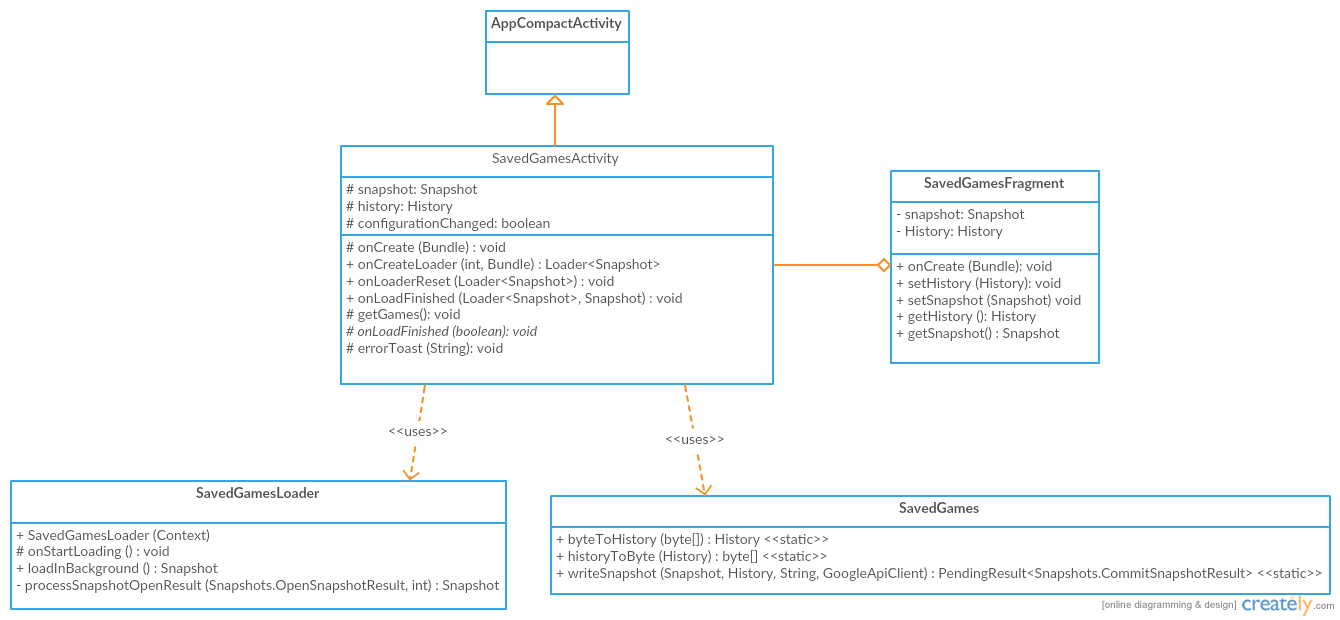
\includegraphics[width=0.9\linewidth]{SavedGamesHierarchy}
	\caption{Saved Games Hierarchy}
	\label{fig:saved-games-hierarchy}
\end{figure}

\texttt{SavedGamesActivity} is a base abstract class implementing the interaction with Saved Games. In order to handle configuration changes it uses a headless fragment, \texttt{SavedGamesFragment}. It also stores a boolean flag set to \texttt{true} when a configuration change occurs. In this way its subclasses are able to recognize that, behaving accordingly. 

To avoid a heavy loading in the UI thread, we use an \texttt{AsyncTaskLoader}, \texttt{SavedGamesLoader}. Following Google's best practices, we handle the possibility of conflicts in Saved Games by loading the most recent instance. Even if we could save more than one \texttt{Snapshot}, we prefer storing just one. This is an opportunistic choice: we have no reason to do otherwise.

We use a bunch of classes implementing \texttt{Serializable} in order to deserialize the blob provided by Google. For this end, we use \texttt{SavedGames}. It is basically a companion class providing static methods for serializing and deserializing bytes. 